\chapter{Il Mondo dei Sogni} \label{cap:mondo-dei-sogni}

Ogni persona ha almeno un sogno ogni notte.
Alcuni sogni vengono dimenticati immediatamente al risveglio, altri vengono ricordati per mesi o addirittura anni.
I loro contenuti vanno dal curiosamente bizzarro all'iperrealistico, dall'incredibilmente bello all'indicibilmente
terrificante.
Per questi motivi, l'umanità è stata affascinata dal mondo dei sogni fin dagli albori della storia documentata.
Nel campo scientifico, tre principali approcci si sono differenziati tra loro nello studio dei sogni, essi sono
l'approccio psicoanalitico, neurofisiologico e psicologico.

Le esperienze che costituiscono il sogno emergono casualmente dal cervello, oppure affiorano in base a determinati
parametri?
I sogni hanno un significato?
Qual è o quali sono le funzioni del sognare?
Lo scopo della psicoanalisi è quello di fornire ipotesi per rispondere a queste domande.

L'approccio neuropsicologico è invece interessato alla fenomenologia dei sogni e alla sua relazione con l'attività
cerebrale, concentrandosi sul come le informazioni vengano elaborate durante il sonno e sul ruolo delle varie regioni
cerebrali specializzate rispetto all'esperienza onirica.

Infine, l'approccio psicologico si concentra su una ricerca orientata da aree di interesse quali
la natura e la descrizione dei sogni, i fattori che influenzano il contenuto dei sogni e l'influenza dei sogni sulla
vita diurna.

In questo breve capitolo si cercherà di dare una concisa panoramica generale sul mondo dei sogni, integrando le diverse
prospettive sopra citate e attingendo da informazioni provenienti da svariati studi scientifici che hanno contribuito
a descrivere lo stato dell'arte attuale in questo campo ~\cite{Ruby2011ExperimentalRO, Akhtar2022, Schredl2005}.


\section{Perché sogniamo?}
Sebbene le scienze mediche abbiano fatto enormi progressi negli ultimi sessantacinque nell'intento di comprendere il
sonno e le relative attività cerebrali, medici e scienziati non sono ancora riusciti a spiegare con esattezza la
natura e le ragioni del sogno.
Questo è il motivo per cui i sogni sono ancora ritenuti un campo di ricerca misterioso ed affascinante: non esiste
tutt'ora una loro spiegazione univoca e condivisa.

Prima di tentare di comprendere i sogni, però, è fondamentale che si conoscano i meccanismi del sonno.
Il sonno non è uniforme.
Durante la notte, la totalità del periodo di sonno può essere scomposta in diversi cicli, ciascuno dei quali è
composto da una sequenza di quattro fasi principali.
In una notte tipica, una persona attraversa da quattro a sei cicli di sonno.
Non tutti i cicli di sonno hanno la stessa durata, tuttavia, essa si attesta attorno ad una media di 90 minuti per
ciascuno.

\begin{figure}[t]
    \centering
    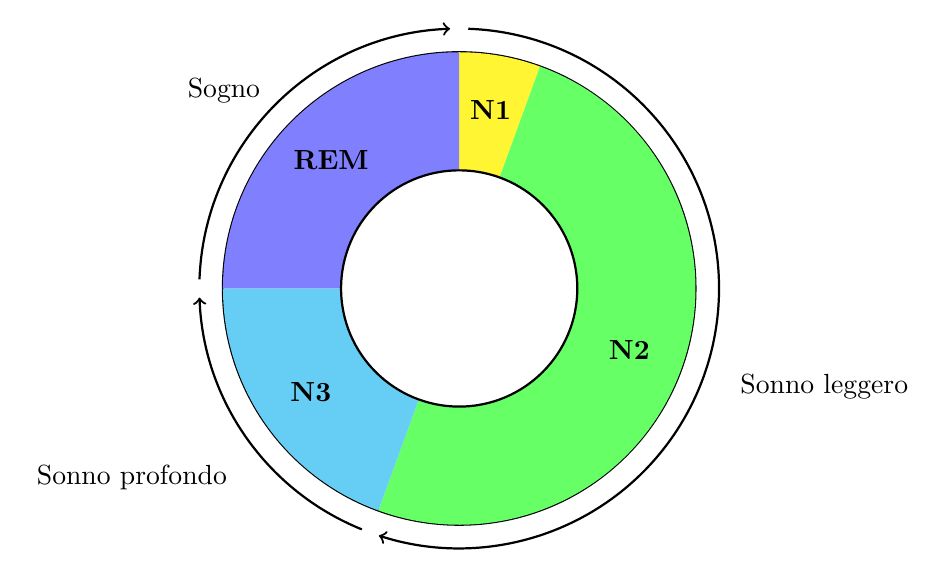
\begin{tikzpicture}

% Circle base
\draw[thick] (0,0) circle (3cm);

% Sectors
% Sectors
\fill[yellow!80] (0,0) -- (90:3cm) arc[start angle=90, end angle=70, radius=3cm] -- cycle;
\fill[green!60] (0,0) -- (70:3cm) arc[start angle=70, end angle=-110, radius=3cm] -- cycle;
\fill[cyan!60] (0,0) -- (250:3cm) arc[start angle=250, end angle=180, radius=3cm] -- cycle;
\fill[blue!50] (0,0) -- (180:3cm) arc[start angle=180, end angle=90, radius=3cm] -- cycle;

% Inner circle
\draw[thick, fill=white] (0,0) circle (1.5cm);

% Text
%\node at (0,0) {\text{Ciclo del Sonno}};
\node at (80:2.3cm) {\textbf{N1}};
\node at (340:2.3cm) {\textbf{N2}};
\node at (215:2.3cm) {\textbf{N3}};
\node at (135:2.3cm) {\textbf{REM}};

% Arrows and labels
\draw[->, thick] (88:3.3cm) arc[start angle=88, end angle=-108, radius=3.3cm];
\node at (345:4.8cm) {Sonno leggero};

\draw[->, thick] (248:3.3cm) arc[start angle=248, end angle=182, radius=3.3cm];
\node at (210:4.8cm) {Sonno profondo};

\draw[->, thick] (178:3.3cm) arc[start angle=178, end angle=92, radius=3.3cm];
\node at (140:3.9cm) {Sogno};

\end{tikzpicture}
    \vspace{-10pt}
    \caption{Il ciclo del sonno}
    \label{fig:sleep-cycle}
\end{figure}

Le quattro fasi principali di ogni ciclo sono N1, N2, N3 e REM, acronimo di \textit{Rapid Eye Movement}.
La fase N1 è quella che consiste del sonno più leggero.
Infatti durante questa fase, una persona può essere svegliata facilmente.
Durante la fase N2, le attività neuronali iniziano a rallentare, preparando il nostro corpo per il sonno
profondo.
La fase N3 è conosciuta come sonno profondo.
Durante questa fase i muscoli diventano inattivi e la persona dormiente risulta molto difficile da svegliare.
Accade spesso che le persone che vengono svegliate mentre il loro cervello trova nella fase di sonno profondo
si sentano assonnate e confuse per alcuni minuti, prima di riuscire a svegliarsi completamente.
Queste prime tre fasi compongono il sonno NREM (Non-REM).
Più alta è la fase di sonno NREM, e più sarà difficile svegliare la persona.
Dopo il sonno profondo arriva il sonno REM, la fase del sonno in cui si verificano i sogni.
Durante il sonno REM, il battito cardiaco e la pressione sanguigna aumentano, la respirazione diventa più rapida e
si verifica un rapido movimento degli occhi, da cui il nome di questa fase.
Grazie all'avanzamento delle tecnologie di imaging cerebrale, il ciclo sonno-veglia è stato studiato accuratamente,
a tal punto che ora è possibile identificare in quale delle tre fasi si trova il cervello durante il sonno.
\`E stato dimostrato che il cervello si disattiva globalmente dallo stato di veglia allo stato di sonno NREM,
e successivamente si riattiva durante il sonno REM, in misura maggiore rispetto a quanto avviene durante la veglia.
Nell'identificazione dello stato del cervello ricopre un ruolo importante il riconoscimento del suo stato di coscienza
tra i suoi possibili sotto-stati: la \textit{coscienza primaria} e \textit{la coscienza secondaria}.
La coscienza primaria è la semplice consapevolezza di percezione sensoriali e delle emozioni, nonché la consapevolezza
del mondo, ottenuta attraverso le informazioni avanzate di coordinazione visiva e motoria che il cervello riceve.
La coscienza secondaria è uno stato di coscienza più avanzato avanzato, in quanto include la coscienza primaria,
l'analisi astratta, o il pensiero, e i componenti meta cognitivi, che includono la consapevolezza di essere coscienti.
La maggior parte degli animali mostra determinati livelli di coscienza primaria, ma solo gli esseri umani sono
hanno sperimentalmente dimostrato di possedere la coscienza secondaria. %TODO: Citazione sulla Protocoscienza
Un'altra caratteristica cerebrale che ci distingue dagli altri animali e che inficia sull'esperienza
onirica è la presenza di una corteccia cerebrale molto sviluppata, la parte più esterna del cervello che
gestisce l'apprendimento, il pensiero e l'elaborazione delle informazioni, considerata come uno dei massimi
traguardi dell'evoluzione.
Il sonno REM inizia, infatti, quando una parte del tronco encefalico nota come \textit{ponte} invia un segnale al
talamo, ordinandogli di attivare la corteccia cerebrale.
Questa attivazione della corteccia è la responsabile della nostra consapevolezza primaria durante l'esperienza del
sogno, oltre che del loro ricordo da svegli. \newline

I fatti scientificamente accertati finiscono qui, e tutto ciò che segue sulle ragioni del sognare rimangono teorie.
Esse vengono spesso chiamate ``teorie del sogno'', ve ne sono molteplici e delle più disparate.
A seguire, alcune delle più note e condivise.

\nlparagraph{Ipotesi della continuità}

Un grande numero di studi trattano la così chiamata \textbf{ipotesi della continuità} (in inglese
\textit{Continuity Hypothesis}), la quale afferma che i contenuti nei sogni riflettono le preoccupazioni
e le idee quotidiane dei sognatori, piuttosto che i desideri libidici nascosti o le strategie emotive compensatorie
come Freud e Jung sostenevano.
I contenuti dei sogni sarebbero quindi correlati ad aspetti della vita da svegli o alle variabili psicologiche
dell'individuo.
Ad esempio una persona in uno stato ansioso causato da un esame imminente potrebbe sognare di non passarlo.
Sotto l'ipotesi della continuità, i ricercatori suggeriscono che i sogni sarebbero il risultato di una raccolta di
informazioni e vissuti della vita quotidiana che verrebbero archiviati nella memoria a lungo termine.
Si noti, tuttavia, che la teoria non da spiegazioni sul perché alcuni ricordi vengano
fatti emergere più o meno frequentemente nei sogni, ed essa è stata criticata come una teoria imprecisa.

\nlparagraph{Teoria evolutiva della simulazione}

I sogni potrebbero anche essere il risultato di un adattamento evolutivo.
Teorie del sogno come la \textbf{teoria della simulazione} propongono che lo scopo del sogno è quello di prepararci
al meglio per affrontare i pericoli del mondo reale, come in una sorta di simulazione per i nostri istinti primitivi.
Il sogno può essere visto come una riproduzione della nostra vita sociale o come un modo per prepararci ai pericoli
della vita reale: in questo modo il sogno rappresenterebbe un ambiente sicuro dove far pratica delle nostre
abilità di sopravvivenza e allenare la nostra capacità di affrontare situazioni stressanti, fornendoci un vantaggio
evolutivo.
Questo spiegherebbe perché scenari spaventosi o emotivamente intensi risultano essere oggetto frequente dei sogni:
fuggire da un inseguimento, cadere da un precipizio, presentarsi nudi in un luogo pubblico o dimenticare di studiare
per un esame sono solo alcuni degli esempi condivisi da molti sognatori.

\nlparagraph{Teoria del consolidamento delle memorie}

Secondo la teoria dell'\textbf{auto-organizzazione} (in inglese \textit{Self-Organization Theory}), invece, i sogni
servirebbero principalmente a consolidare ed elaborare le informazioni raccolte durante il giorno appena passato.
Secondo questo modello, quindi, il sogno sarebbe solo un ``effetto collaterale'' dell'attività neuronale
che si verifica durante il sonno nel mentre che il cervello si attiva nel consolidare i ricordi.
La teoria afferma che durante questo processo inconscio i ricordi vengono o rafforzati o indeboliti, a seconda
che essi siano ritenuti utili o meno.
Alcune ricerche danno supporto a questa teoria, in quanto hanno mostrato che le persone migliorano nello svolgere
delle attività complesse quando queste sognano di farle.
Inoltre, il fatto che durante il sonno REM le onde theta a bassa frequenza si siano mostrate essere più attive nel
lobo frontale, proprio come quando le persone imparano, memorizzano e ricordano informazioni da svegli,
sembra confermare questa teoria.

\nlparagraph{Teoria del problem-solving}

Altre teorie sui sogni affermano che il loro scopo sia quello di dare supporto alla nostra capacità di \textbf{risolvere
problemi}.
In accordo ad esse, la parte inconscia della nostra mente si ritroverebbe, durante il sogno, in una dimensione
svincolata, libera di esplorare il suo potenziale creativo, lontana dalle soffocanti realtà del mondo conscio.
Le ricerche hanno infatti dimostrato che sognare promuove efficacemente il pensiero creativo, dandoci l'opportunità
di fare connessioni inaspettate tra ricordi e idee che appaiono nei nostri sogni.

\nlparagraph{Teoria della regolazione emotiva}

La teoria dei sogni sulla \textbf{regolazione emotiva}, invece, afferma che la funzione dei sogni sia quella di aiutarci
a elaborare emozioni e traumi nello spazio sicuro offerto dal sogno.
Ci sono evidenze che mostrano come due organi siano particolarmente attivi durante il sogno: l'amigdala,
responsabile dell'elaborazione delle emozioni, e l'ippocampo, che filtra
le informazioni da spostare dalla memoria a breve termine a quella a lungo termine.
Il forte legame tra il sognare, la memorizzazione e la rielaborazione emotiva aiuterebbe a spiegare perché molti sogni
siano emotivamente intensi e perché le esperienze traumatiche tendono a ripresentarsi nei sogni.
Ci sono anche ricerche che mostrano una connessione tra la capacità di elaborare le emozioni e la quantità di sonno
REM che una persona riceve. \newline

Infine è curioso notare che, sebbene ricada tra le teorie fortemente anti-psicoanalitiche, alla fine del
ventesimo secolo è stata proposta anche la teoria per cui il sogno non avrebbe alcuna reale funzione, ma che,
piuttosto, consisterebbe semplicemente in un epifenomeno del sonno.

Sebbene molte altre teorie siano state proposte, non esiste un consenso univoco su quale teoria del sogno
spieghi la funzione del sogno meglio delle altre, rendendo difficile l'intento di fornire una visione integrata e
soddisfacente dell'incomprensibile mondo dei sogni.

\section{Le forme di sogno}

Per comprende a pieno in quali forme si possono presentare i sogni e cosa permette di distinguerle oggettivamente,
risulta utile analizzare lo stato in cui il cervello può trovarsi durante il sonno.

\nlparagraph{Sogni REM}

Sin da quando emerse l'approccio neuroscientifico alla fine degli anni '50, fu subito proposto il modello di un
substrato fisiologico del sogno: il sonno REM.
Quando si entra in sonno REM, il cervello cambia completamente a livello neurochimico, risultando in un'attivazione
cerebrale molto più intensa rispetto allo stato di veglia.
Tale attivazione avviene nella parte del cervello chiamata sistema limbico, dove si trova
l'amigdala, direttamente correlata al contenuto intensamente emotivo dei sogni.
Assieme all'amigdala, anche l'ippocampo e la corteccia cingolata anteriore risultano particolarmente attivi,
i quali, insieme, costituiscono l' ``asse della paura'' del cervello e dei ricordi ad essa legati.
Di fatti, differenze in termini di tessuto cerebrale di ippocampo e amigdala tra singoli individui si sono dimostrate
essere correlate a differenze nei loro sogni in termini di conenuto emotivo e stravaganza.

Al contempo la corteccia prefrontale, sede del pensiero razionale e del ragionamento critico, tipicamente non
partecipa all'attività cerebrale durante il sogno.
Questo spiega perché lo svolgimento di un sogno può risultare assurdo o privo di logica e che, nonostante questo,
tutto risulti normale per il sognatore.
Nello specifico, il risultato di tale natura nel contenuto dei sogni è dovuto alla completa disattivazione della
corteccia prefrontale dorsomediale, motivo per cui solo rare volte i resoconti dei sogni parlano di matematica.

Molti studi hanno anche rivelato una forte attivazione della corteccia visiva occipito-temporale superiore durante
il sonno REM, aspetto coerente con la vivida immaginazione visiva dei sogni.
Mentre la corteccia visiva primaria, responsabile per la ricezione dei segnali visivi dal mondo esterno, rimane a
riposo, la corteccia visiva secondaria, che aiuta ad elaborare e interpretare quei segnali, rimane attiva.
L'immaginario dei sogni nasce, probabilmente, dal tentativo della corteccia visiva secondaria di decifrare ed unire in
una visione coerente i segnali che le vengono inviati, molti dei quali sono generati internamente.
Oltre a quelle della visione, anche altre regioni legate alla percezione e al movimento rimangono attive, motivo
per cui il movimento è un elemento ricorrente nei sogni.
Naturalmente un'altra regione, nel tronco encefalico, paralizza la maggior parte del corpo, impedendo al sognatore di
agire fisicamente durante il sogno.

\nlparagraph{Sogni NREM}

A seguito della scoperta del sonno REM, i sogni erano ritenuti essere un fenomeno esclusivo di questa fase.
Sin dagli anni '60, tuttavia, questa ipotesi fu messa in discussione, per via di evidenze che mostravano che
alcune caratteristiche dei report dei sogni non potevano essere spiegate con il modello proposto.
\`E grazie a successive valutazioni in ambito neurofisiologico, psicofisiologico e, più recentemente,
grazie a tecniche di neuroimaging, che si è potuto scoprire che i sogni avvengono anche durante il sonno NREM,
in particolare, attorno alla sua prima e ultima fase. %TODO:  Rapid eye movement sleep, non-rapid eye movement sleep, dreams, and hallucinations.
Questo ha portato a riconsiderare la natura dei sogni, indicando che essi non sono limitati né causati dai meccanismi
che controllano il sonno REM, e che potrebbero esistere aree cerebrali associate ai sogni completamente diverse.
Tuttavia l'attenzione della maggior parte degli studi sui sogni ha continuato a concentrarsi sui sogni REM poiché,
in tale fase, essi sono più frequenti, più lunghi e più vividi, oltre che avere contenuti più bizzarri.
Sebbene le differenze tra le due tipologie di sogno siano ancora oggetto di dibattito, esiste un consenso generale
sulla possibilità di distinguere i report di sogni REM da quelli NREM: maggior numero di parole usate,
contenuti emotivi intensi, e maggiore multi-sensorialità percettiva sono elementi distintivi dei sogni REM,
mentre i sogni NREM si attengono maggiormente alla propria vita da svegli e sono spesso più simili a
processi di pensiero.

\nlparagraph{Sogni lucidi}

I sogni lucidi sono definiti come sogni in cui il sognatore è consapevole di star sognando, il quale, spesso, ha
qualche forma di controllo sul contenuto del sogno stesso.
Se normalmente lo stato di coscienza del sogno è considerato essere uno stato di coscienza primaria,
i sognatori lucidi sarebbero in grado di sperimentare coscienza primaria e secondaria simultaneamente, ma comunque
in modo separato.
Mentre le esperienze del sogno si collocano nella coscienza primaria, il sognatore che
riconosce il sogno può dirsi dotato di una forma di coscienza secondaria, in quanto è consapevole del proprio
stato mentale.
Degli studi effettuati attraverso elettroencefalogramma, infatti, hanno mostrato che il sogno lucido si colloca a metà
tra i due stati. %TODO: The neurobiology of consciousness: Lucid dreaming wakes up, International Journal of Dream Research, 2(2), 41–44
D'altra parte, questa forma di sogno è relativamente rara: si stima che circa il 50\% delle persone abbia avuto almeno
un sogno lucido nella propria vita, mentre solo il 10\% circa ne ha almeno due al mese.
Il motivo per cui alcune persone sperimentano sogni lucidi più frequentemente di altre è tutt'ora ignoto, sebbene
si sappia che le regioni prefrontali e parietali del cervello svolgano un ruolo determinante in tale fenomeno.

\nlparagraph{Incubi}

Con incubi si intendono i sogni caratterizzati da forti emozioni negative, come paura, ansia, tristezza o rabbia.
Essi sono una sotto-tipologia di sogni REM, sebbene si sia osservato che gli incubi post-traumatici possano
verificarsi anche durante il sonno NREM.
Essendo molto comuni, le motivazioni che gli esperti forniscono per la loro comparsa ricadono su alcune delle
teorie del sogno viste in precedenza, come l'ipotesi della continuità, la teoria evolutiva della simulazione e
la teoria della regolazione emotiva.
Tuttavia si è potuto notare che gli incubi siano strettamente legati alla salute mentale del sognatore: persone
che soffrono di disturbo post-traumatico da stress, ad esempio, spesso presentano incubi che si presentano con
maggiore frequenza e intensità.
Questi sogni potrebbero infatti essere, in generale, il risultato di un tentativo del cervello di elaborare e superare
le le esperienze stressanti e le emozioni negative vissute durante la veglia.

\section{Come si catturano i sogni}

Il sogno, sebbene sia un fenomeno di forte natura soggettiva, può essere immortalato in un racconto o resoconto
narrativo che ne spieghi il contenuto.
In ambito scientifico, la definizione condivisa dalla più ampia fetta di ricercatori è che un sogno
(o il report di un sogno) è ``la rievocazione di un'attività mentale che è avvenuta durante il sonno''.
\`E importante notare che il sognare, come attività mentale durante il sonno, non è direttamente misurabile,
poiché prima che la persona possa riportare l'esperienza avvenuta durante il sonno, essa
deve passare attraverso il passaggio dallo stato di sonno a quello di veglia, assieme alla differenza di tempo
che ne consegue.
Questo aspetto porta al \textbf{problema della validità}, che consiste nel chiedersi se il resoconto del sogno sia
un'adeguata rappresentazione dell'effettiva esperienza del sogno.
Problemi legati alla dimenticanza del sogno sono comuni, e potrebbero portate il soggetto a fornire più informazioni
di quelle effettivamente sperimentate, o a riportare eventi in ordine diverso da quello in cui sono avvenuti.
Il resoconto di un sogno, infatti, essendo puramente narrativo, potrebbe riscontrare delle difficoltà nel
descrivere la sua visione d'insieme, e al contempo rendere difficile la descrizione qualitativa dell'esperienza
che può includere oggetti irreali, sensazioni bizzarre o emozioni.
Ciò che si può affermare con più sicurezza, invece, è che il resoconto del sogno riflette l'attività mentale
sperimentata durante il sonno piuttosto che essere solamente un prodotto del processo di risveglio: grazie ad una
combinazione degli approcci fisiologici con l'analisi del contenuto dei sogni, è stato possibile dimostrare che i
resoconti dei sogni corrispondono parzialmente ai parametri fisiologici registrati durante il sonno REM, come i
movimenti oculari e la frequenza cardiaca. \newline

In ogni caso, i racconti riportati dai sognatori rimangono il principale strumento per l'analisi dei sogni
in ambito scientifico, rendendolo un ambito di ricerca complesso e pieno di dati testuali non strutturati.
Nell'ambito della ricerca, questi resoconti sono raccolti a partire dal sognatore attraverso due principali
forme, la forma scritta e la forma vocale.
Per forma scritta si intendono tutti quei resoconti trascritti su carta o su un sistema informatico
direttamente dal sognatore.
Questo è il caso in cui, tipicamente, siano stati raccolti dal sognatore sotto forma di diario personale,
portando spesso a grandi collezioni di sogni personali derivanti da periodi di tempo più o meno prolungati.
Con forma vocale, invece, si intendono i resoconti raccolti attraverso interviste o registrazioni audio fatte
dall'analista, i quali vengono poi trascritti.
Questa modalità di raccolta dei sogni è spesso utilizzata in ambito clinico, dove il sognatore è guidato da un
terapeuta a descrivere il proprio sogno, oppure negli studi di laboratorio, dove il sognatore è invitato
a raccontare un sogno recente.
Sicuramente si tratta della modalità più indicata quando l'obiettivo è quello di ridurre al minimo il problema
della validità precedentemente menzionato: gli studi aumentano la loro validità quando il sogno viene raccontato
non appena sperimentato, quindi al seguito immediato di un risveglio dalla fase REM o NREM.

I metadati che accompagano i testi dei sogni, consistono di dati ulteriori che il più delle volte possono consistere
delle generalità del sognatore e la data del sogno.
Nel caso di studi clinici, possono essere abbinate anche informazioni riguardanti la salute mentale del sognatore o
altri dati provenienti da questionari standard. \newline

\`E in questo contesto che si colloca \textit{Sogniario} \footnote{https://sogniario.unicam.it/}
(nome derivato dalla sintesi di sogni e diario), l'applicazione sviluppata dal gruppo di ricerca del prof.
Michele Bellesi dell'Università di Camerino, nata da una collaborazione tra il Brain and Sleep Research Laboratory
della medesima istituzione e il Molecular Mind Laboratory della Scuola IMT Alti Studi Lucca.
Il principale scopo di Sogniario è quello costruire un corposo archivio di report di sogni per assistere medici e
ricercatori nello studio dei sogni.
In questo caso i vantaggi di entrambi i metodi di raccolta dei sogni vengono sfruttati:
un gran numero di report di sogni in forma vocale possono essere raccolti da una vasta popolazione di sognatori,
utilizzando la trascrizione vocale automatica fornita dall'applicazione.
Oltre alle generalità dei sognatori, i metadati da accompagnare ai report dei sogni raccolti da Sogniario
comprendono anche questionari relativi al sonno, come i questionari sul cronotipo
(\textit{Morningness-Eveningness Questionnaire}, MEQ) o sulla qualità del sonno
(\textit{Pittsburgh Sleep Quality Index}, PSQI).
Iniziative come queste permettono quindi di aprire le porte alla ricerca sui report di sogni su larga scala, con
l'opportunità di sfruttare tecniche tipicamente applicabili a grandi moli di dati non strutturati per
estrapolare possibili fattori predittivi dello stato di salute cognitivo ed emotivo dei sognatori.

\section{Analisi dei sogni e ricadute sulla salute}

All'inizio del ventesimo secolo, Freud presentò il concetto di inconscio.
Egli propose che una parte della nostra mente è costituita da pensieri, desideri, emozioni e conoscenze di cui non
siamo consapevoli, ma che influenzano e guidano profondamente i nostri comportamenti.
Propose, inoltre, che l'inconscio potesse emergere attraverso lapsus e sogni.
Per questi motivi, secondo Freud, decodificare i sogni attraverso il metodo della libera associazione poteva
fornire accesso a ciò che rende ognuno di noi speciali, svelare i moventi che guidano il nostro comportamento e
fornire accesso a una dimensione sconosciuta di noi stessi.
Questa ipotesi, che attribuisce importanza al significato dei sogni, è stata raramente considerata seriamente
dagli neuroscienziati, che spesso considerano la teoria di Freud come non scientifica.

Oggi, lo scopo principale dell'analisi del contenuto dei sogni è la quantificazione di loro specifici aspetti,
come potrebbero essere le persone che vi appaiono, le interazioni che avvengono o i luoghi in cui si svolgono,
allo scopo di effettuare delle analisi statistiche.
Ad esempio, potrebbero essere condotti degli studi in cui, a partire dall'ipotesi di uno psicologo, si vuole
vedere se la tematica del rifiuto appare più spesso in soggetti afflitti da depressione rispetto a un gruppo
di persone sane.
Questi esperimenti, a partire da una precisa metrica che quantifica la presenza di tale tematica nei
sogni, sono condotti su gruppi di persone, e i loro sogni sono valutati in base a tale metrica.
Sebbene si sia dimostrato che i contenuti dei sogni siano correlati allo stato umorale, al tempo
dedicato a particolari attività intraprese dal sognatore durante la giornata ed ai tratti della personalità,
molte evidenze suggeriscono che siano intimamente interrelati allo stato di benessere psicologico dell'individuo.
Disturbi della psiche come la depressione, l'ansia, la schizofrenia, la depressione, il bipolarismo e
il disturbo post-traumatico da stress dimostrano di avere un impatto significativo sui contenuti dei sogni,
che assumono con maggiore frequenza la forma di incubi o altre forme generalmente angosciose.

Ad esempio, studi su report di pazienti schizofrenici hanno mostrato che i loro sogni sono
caratterizzati da un aumento della frequenza di sconosciuti maschi, interazioni sociali più aggressive ed
emozioni più ansiose. % TODO: Dreams and schizophrenia. Arch Gen Psychiatry
L'analisi formale dei sogni può comprendere anche una valutazione dettagliata di altre caratteristiche del report
oltre al contenuto, come l'aspetto generale, il flusso del discorso, la chiarezza, l'orientamento nel tempo,
nello spazio e nella persona, la stravaganza, l'intreccio della narrazione e la logica.
Ad esempio, il livello di stravaganza potrebbe essere definito e misurato come il numero di oggetti, persone o
luoghi che appaiono avere un certo insieme di caratteristiche apparentemente incoerenti.
Tuttavia questo parametro in particolare, non si è rivelato particolarmente utile per distinguere i sogni di
soggetti psicotici da quelli di soggetti sani, principalmente per via del fatto che la stravaganza è un aspetto
dovuto alla normale disattivazione della corteccia prefrontale dorsomediale durante il sonno REM.

Altri aspetti, legati all'intreccio e al flusso del discorso sono risultati essere più promettenti.
Analisi relativamente più recenti eseguite sul grafo delle parole dei report hanno mostrato che i sogni di soggetti con
schizofrenia e disturbo bipolare possono variare significativamente rispetto a quelli di soggetti sani,
oltre che tra i singoli individui~\cite{mota2014graph}.
Gli aspetti semantici e grammaticali che sono stati analizzati includono la frequenza delle parole, la presenza di
cicli di parole ricorrenti, la connettività delle parole e la loro organizzazione in componenti
fortemente connesse.
Curiosamente, l'analisi ha mostrato che tali differenze potessero essere colte solamente attraverso il racconto di
sogni, e non di esperienze di veglia, quasi a suggerire che, come Freud sosteneva, i sogni possano essere un mezzo più
efficace per esplorare le differenze tra individui.